% !TeX spellcheck = en_US
% !TeX program = xelatex

\documentclass[a4paper,12pt]{article}
\renewcommand{\baselinestretch}{1.5}
\usepackage[utf8]{inputenc}
\usepackage[T2A, T1]{fontenc}
\usepackage[english, russian]{babel}

\usepackage{fontspec}
\setmainfont{Times New Roman}
\usepackage{setspace,amsmath}
\usepackage{amssymb}
\usepackage{dsfont}

\makeatletter
\let\@fnsymbol\@arabic
\makeatother

\usepackage{geometry}
\geometry{
a4paper,
total={170mm, 257mm},
left=20mm,
top=20mm,
}

\usepackage{systeme}
\usepackage{skak}
\usepackage{mathtools}
\usepackage{unicode-math}
\usepackage{array}
\usepackage{makecell}
\usepackage{subfiles}
\usepackage{hyperref}
\hypersetup{pdfstartview=FitH, linkcolor=blue, urlcolor=blue, colorlinks=true}
\usepackage{framed}
\usepackage{graphicx}
\usepackage{caption}
\usepackage{subcaption}
\usepackage{color}
\usepackage{chngcntr}

\usepackage{float}
\floatstyle{plaintop}
\usepackage{enumitem}
\setlength{\parindent}{0pt}

\graphicspath{{./img/}}
\newcommand{\myPictWidth}{.95\textwidth}
\newcommand{\phm}{\phantom{-}}
\newcommand{\beq}{\begin{equation}}
\newcommand{\eeq}{\end{equation}}


\begin{document}
Muravtsev Alexander 5040103/10401.

Basic kinematics and geometry. Virtual displacement.
\section{Basic kinematics and geometry}
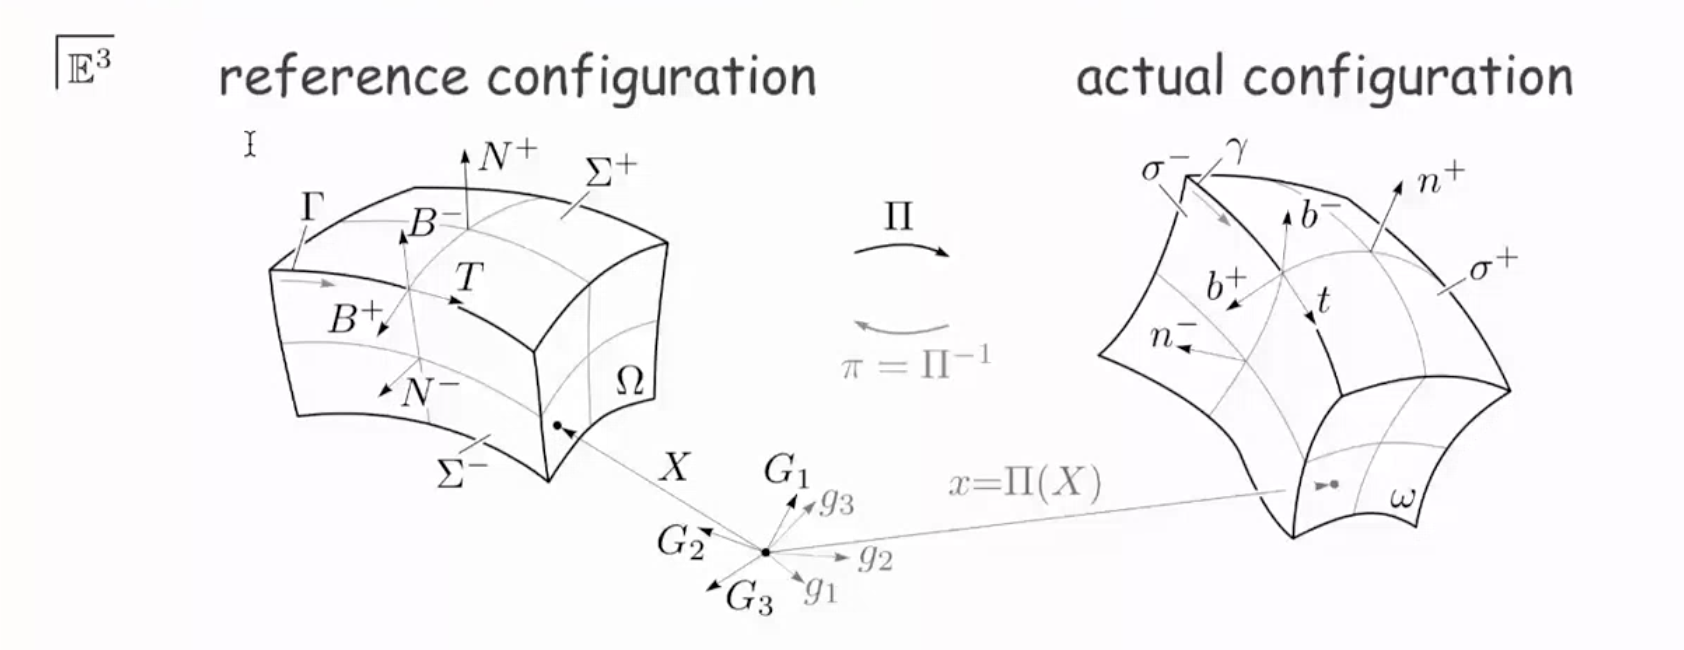
\includegraphics[width=\textwidth]{ReferenceActualConfigurations}
Reference configuration = Lagrangian configuration (Lagrange prefer to study everything in reference configuration)

Actual configuration = Eulerian configuration (Euler was studying the flow of fluids in actual configuration)

When body has edges and wedges the analysis of contact interactions is changing dramatically. So in the theory of second gradient materials it is necessary to be very carefully specifying the shape of the body in reference configuration and inside this shape not only faces must be included but also edges and wedges.

$N^+$ is the normal to the top face $\Sigma^+$.

$\Gamma$ is the edge (curve that is in common with $\Sigma^+$ and $\Sigma^-$ surfaces)

$N^-$ is the normal to face $\Sigma^-$.

$T$ is the unit tangent vector to the curve $\Gamma$. $B^+$ is the tangent vector to $\Sigma^+$. $B^+$ is normal to $T$ so we call it as unit normal vector to the curve $\Gamma$. 

Similarly we can define vector $B^-$: it is normal to $T$ and is the tangent vector to $\Sigma^-$.

\textbf{Assumptions:} consider suitably regular placement. We have placement $\Pi$ which is not allowing new edge formation. So an edge becomes an edge, a wedge becomes a wedge and a face is transformed to another face.

In the language of differential geometry $\Pi$ is a diffeomorphism of class $C_1$ at least ($\Pi$ have all partial derivatives which are continuous). For instance, we can not describe crack formation in this theory (new edges are created during crack formation; $\Pi$ is discontinuous in the localisation of crack).

$\Pi$ placement: $\Sigma^+$ is mapped to $\sigma^+$, $N^+$ is mapped to $n^+$ and so on.

\beq\label{PiTransform}
\Pi: \Omega\rightarrow\mathbb{E}^3\,\,\,\,\,\,\,X\mapsto x=\Pi^i(X)g_i
\eeq

Expression in \eqref{PiTransform} is written in Einstein notation:
\beq
\Pi^i(X)g_i=\sum\limits_{i=1}^3\Pi^i(X)g_i
\eeq

First gradient of placement (partial derivative of $\Pi^i$ with respect to $X$):
\beq
F_A^i=(\nabla\Pi)_A^i=\frac{\partial\Pi^i}{\partial X^A}
\eeq
(the second order tensor: 1 time Lagrangian and 1 time Eulerian -- index $i$ is saturated with vectors $g_i$ in actual configuration according to \eqref{PiTransform}; while index A refers to the reference configuration)


Second gradient of placement:
\beq
F_{AB}^i=(\nabla F)_{AB}^i=\frac{\partial^2\Pi^i}{\partial X^A\partial X^B}
\eeq
(the third order tensor: 2 times Lagrangian and 1 time Eulerian -- index $i$ is saturated with vectors $g_i$ in actual configuration according to \eqref{PiTransform}; while A and B indices refer to the reference configuration)

\newpage

\section{Virtual displacement}
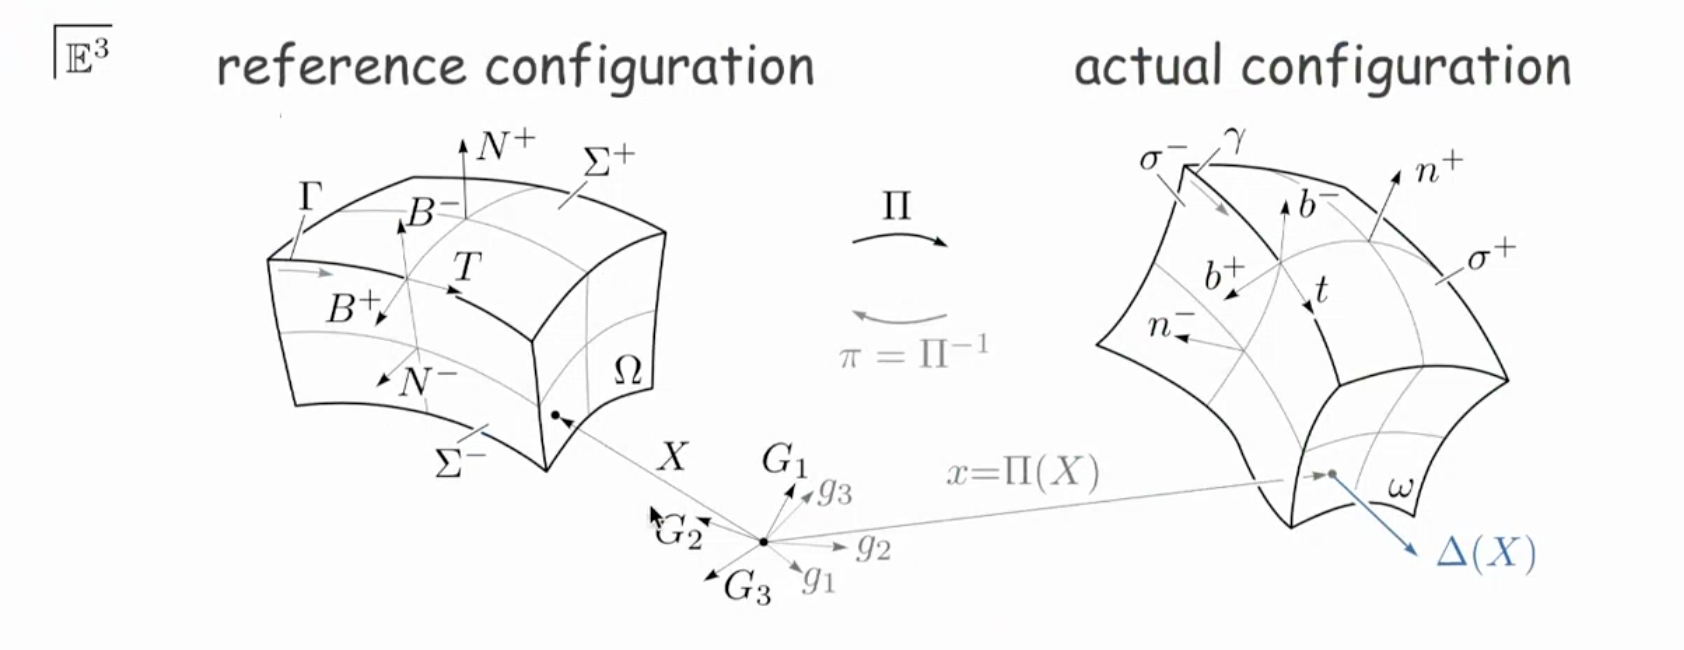
\includegraphics[width=\textwidth]{VirtualDisplacement}

The virtual displacement is a small variation of the placement $\Pi$:
\beq
\Delta(X)=\Delta^i(X)g_i=\delta\Pi^i(X)g_i
\eeq

$X$ is an independent variable; $\Delta$ is a small variation of the placement, so virtual displacement is a small Eulerian vector.

The first gradient of virtual displacement:
\beq
\delta F_A^i=\frac{\partial\Delta^i}{\partial X^A}
\eeq
(the second order tensor: 1 time Lagrangian and 1 time Eulerian -- index $i$ is saturated with vectors $g_i$ in actual configuration according to \eqref{PiTransform}; while index A refers to the reference configuration)

The second gradient of virtual displacement:
\beq
\delta F_{AB}^i=\frac{\partial^2\Delta^i}{\partial X^A\partial X^B}
\eeq
(the third order tensor: 2 times Lagrangian and 1 time Eulerian -- index $i$ is saturated with vectors $g_i$ in actual configuration according to \eqref{PiTransform}; while A and B indices refer to the reference configuration)

\end{document}
